\documentclass[11pt]{article}
\usepackage[scaled=0.92]{helvet}
\usepackage{geometry}
\geometry{letterpaper,tmargin=1in,bmargin=1in,lmargin=1in,rmargin=1in}
\usepackage[parfill]{parskip} % Activate to begin paragraphs with an empty line rather than an indent %\usepackage{graphicx}
\usepackage{amsmath,amssymb, mathrsfs,  mathtools, dsfont}
\usepackage{tabularx}
\usepackage{tikz-cd}
\usepackage[font=footnotesize,labelfont=bf]{caption}
\usepackage{graphicx}
\usepackage{xcolor}
%\usepackage[linkbordercolor ={1 1 1} ]{hyperref}
%\usepackage[sf]{titlesec}
\usepackage{natbib}
\usepackage{../../Tianpei_Report}

%\usepackage{appendix}
%\usepackage{algorithm}
%\usepackage{algorithmic}

%\renewcommand{\algorithmicrequire}{\textbf{Input:}}
%\renewcommand{\algorithmicensure}{\textbf{Output:}}



\begin{document}
\title{Lecture 10: Vector Bundles}
\author{ Tianpei Xie}
\date{Oct. 16th., 2022}
\maketitle
\tableofcontents
\newpage
\section{Vector Bundles}
\subsection{Definitions}
\begin{itemize}

\begin{figure}[htb]
\centering
\begin{minipage}{0.5\linewidth}
 \centerline{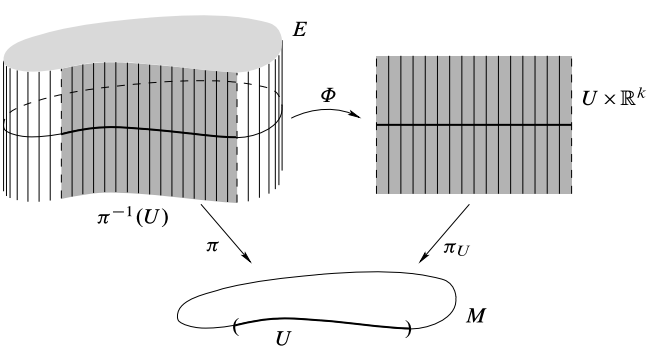
\includegraphics[scale = 0.45]{local_trivialization.png}}
\end{minipage}
\caption{\scriptsize
\textbf{The local trivialization of vector bundle $E$ over neighborhood $U$. \citep{lee2003introduction} }}
\label{fig: local_trivialization}
\end{figure}



\item \begin{definition}
Let $M$ be a \emph{topological space}. A \emph{(real) \underline{\textbf{vector bundle}} of \underline{rank $k$} over $M$} is a \emph{\textbf{topological space}} $E$ together with a \emph{\textbf{surjective continuous} map} $\pi: E \rightarrow M$ satisfying the following conditions:
\begin{enumerate}
\item For each $p \in M$, the \underline{\emph{\textbf{fiber}}} $E_{p} = \pi^{-1}(p)$ over $p$ is endowed with the structure of a \emph{\underline{$k$-dimensional} real \underline{\textbf{vector space}}}.
\item For each $p \in M$, there exist a neighborhood $U$ of $p$ in $M$ and a \emph{\textbf{homeomorphism}} $\Phi: \pi^{-1}(U) \rightarrow U \times \bR^k$ (called \emph{a \underline{\textbf{local trivialization}} of $E$ over $U$}), satisfying the following conditions (Fig. \ref{fig: local_trivialization}):
\begin{enumerate}
\item $\pi_{U}\circ \Phi = \pi$ (where $\pi_U: U \times  \bR^k \rightarrow U$ is the \emph{\textbf{projection}});
\item for each $q \in U$, the \emph{restriction} of $\Phi$ to $E_q$ is a \emph{\textbf{vector space}} \emph{\textbf{isomorphism}} from
$E_q$ to $\set{q} \times \bR^k \simeq \bR^k$.
\end{enumerate}
\end{enumerate}
The space $E$ is called \emph{\textbf{the total space of the bundle}}, $M$ is called its \emph{\textbf{base}}, and $\pi$ is its \emph{\textbf{projection}}. 
\end{definition}

\item \begin{definition}
If $M$ and $E$ are smooth manifolds with or without boundary, $\pi$ is \emph{a smooth map}, and \emph{the local trivializations} can be chosen to be \emph{diffeomorphisms}, then $E$ is called \emph{a \textbf{smooth vector bundle}}. In this case, we call \emph{any local trivialization} that is a \emph{diffeomorphism} onto its image \emph{a \textbf{smooth local trivialization}}.
\end{definition}


\item \begin{remark}
\emph{\textbf{Vector bundle}} $E$ is a \emph{\textbf{generalization and abstraction}} of \emph{\textbf{the tangent bundle}} $TM = \bigsqcup_{p\in M}T_{p}M$. Like the tangle bundle,  the \emph{\textbf{natural coordinates}} constructed on a vector bundle make it look, \emph{locally}, like \emph{\textbf{the Cartesian product}} of \emph{an open subset} of $M$ with $\bR^n$. 
\end{remark}


\item \begin{remark}
The map $\pi$ associates each \emph{vector space} $\pi^{-1}(p)$ in the \emph{vector bundle} to a point $p$ in the topological space $M$. Since $\pi = \pi_{U} \circ \Phi$, we can think of it as a \emph{\textbf{projection map}} after \emph{local trivialization}.
\end{remark}

\item \begin{remark}
The \emph{\textbf{rank}} of a vector bundle is the \emph{\textbf{dimension}} of \emph{vector space} $\pi^{-1}(p)$ associated with each point $p$.
\end{remark}

\item \begin{remark}
A \emph{\textbf{rank-1 vector bundle}} is often called \emph{\textbf{a (real) line bundle}}. \emph{\textbf{Complex vector bundles}} are defined similarly, with ``real vector space" replaced by ``complex vector space" and $\bR^k$ replaced by $\bC^k$ in the definition. 
\end{remark}

\item \begin{remark} Strictly speaking, a vector bundle is a pair $(E, \pi)$ of total space and the projection.  Depending on what we wish to emphasize, we sometimes omit some of the ingredients from the notation, and write ``\emph{\textbf{$E$ is a vector bundle over $M$}},'' or ``\emph{\textbf{$E \rightarrow M$ is a vector bundle}},'' or ``\emph{\textbf{$\pi: E \rightarrow M$ is a vector bundle}}''.
\end{remark}

\item \begin{definition}
If there exists \emph{a local trivialization} of $E$ over \emph{\textbf{all of $M$}} (called \emph{a \textbf{global trivialization} of} $E$), then $E$ is said to be \emph{a \textbf{trivial bundle}}. In this case, $E$ itself is \emph{\textbf{homeomorphic}} to the \emph{product space} $M \times \bR^k$. 

If $E \rightarrow M$ is a \emph{smooth bundle} that admits \emph{a smooth global trivialization}, then we say that $E$ is \emph{\textbf{smoothly trivial}}. In this case $E$
is \emph{\textbf{diffeomorphic}} to $M \times \bR^k$, not just \emph{homeomorphic}. 
\end{definition}
For brevity, when we say that \emph{a smooth bundle} is \emph{trivial}, we always understand this to mean \emph{smoothly trivial}, not just trivial in the topological sense.


\item \begin{lemma} (\textbf{Transition between Two Smooth Local Trivializations})\\
Let $\pi: E \rightarrow M$ be a smooth vector bundle of rank $k$ over $M$. Suppose $\Phi: \pi^{-1}(U) \rightarrow U \times \bR^{k}$ and $\Psi: \pi^{-1}(V) \rightarrow V \times \bR^{k}$ are \textbf{two smooth local trivializations} of $E$ with $U \cap V \neq \emptyset$. There exists a \textbf{smooth map} $\tau:  U \cap V \rightarrow GL(k, \bR)$
such that the composition $\Phi \circ \Psi^{-1}: (U \cap V )\times \bR^k \rightarrow (U \cap V) \times \bR^k$ has the form
\begin{align*}
\Phi \circ \Psi^{-1}(p,v)  &=  (p,  \, \tau(p)v),
\end{align*} where $\tau(p)v$ denotes the usual action of the $k\times k$ matrix $\tau(p)$ on the vector $v \in \bR^k$.
\end{lemma} Note that the following diagram commute:
\[
  \begin{tikzcd}
     (U \cap V )\times \bR^k  \arrow[swap]{dr}{\pi_1} & \arrow[swap]{l}{\Psi}  \pi^{-1}(U \cap V) \arrow{r}{\Phi} \arrow[swap]{d}{\pi} &  (U \cap V )\times \bR^k   \arrow{dl}{\pi_1}\\
    & U \cap V &
  \end{tikzcd}
\] 
\begin{definition}
The smooth map $\tau:  U \cap V \rightarrow GL(k, \bR)$ described in this lemma is called the \underline{\emph{\textbf{transition function}}} between the local trivializations $\Phi$ and $\Psi$. 

For example, if $M$ is a smooth manifold and $\Phi$ and $\Psi$ are the local trivializations of tangent bundle $TM$ associated with two different smooth charts, then the transition function between them is \emph{\textbf{the Jacobian matrix}} of the \emph{coordinate transition map}.
\end{definition}

\item Like the tangent bundle, vector bundles are often most easily described by giving \emph{\textbf{a collection of vector spaces}}, one for each point of the base manifold. The next lemma shows that in order to construct a smooth vector bundle, it is sufficient to construct the local trivializations, as long as they overlap with smooth transition
functions. 
\begin{lemma} (\textbf{Vector Bundle Chart Lemma}). \citep{lee2003introduction} \\
Let $M$ be a smooth manifold with or without boundary, and suppose that for each $p \in M$ we are given a \textbf{real vector space} $E_p$ of some fixed dimension $k$. Let $E = \bigsqcup_{p\in M} E_p$, and let $\pi: E \rightarrow M$ be the map that takes each element of $E_p$ to the point $p$. Suppose furthermore that we are
given the following data:
\begin{enumerate}
\item an \textbf{open cover} $\set{U_{\alpha}}_{\alpha \in A}$ of $M$
\item for each $\alpha \in A$, a \textbf{bijective} map $\Phi_{\alpha}: \pi^{-1}(U_{\alpha}) \rightarrow U_{\alpha} \times \bR^k$ whose restriction to each $E_p$ is a vector space \textbf{isomorphism} from $E_p$ to $\set{p} \times \bR^k \simeq \bR^k$
\item for each $\alpha, \beta \in A$  with $U_{\alpha} \cap U_{\beta} \neq \emptyset$, a smooth map $\tau_{\alpha, \beta}: U_{\alpha} \cap U_{\beta} \rightarrow  GL(k, \bR)$ such that the map $\Phi_{\alpha} \circ \Phi_{\beta}^{-1}$ from $(U_{\alpha} \cap U_{\beta}) \times \bR^k$ to itself has the form
\begin{align}
\Phi_{\alpha} \circ \Phi_{\beta}^{-1}(p,v)  &=  (p,  \, \tau_{\alpha, \beta}(p)v),  \label{eqn: change_of_coordinate_vector_bundle}
\end{align}
\end{enumerate}
Then $E$ has a \textbf{unique topology} and \textbf{smooth structure} making it into \textbf{a smooth manifold} with or without boundary and a \textbf{smooth rank-$k$ vector bundle over M}; with $\pi$ as \textbf{projection} and $\set{(U_{\alpha}, \Phi_{\alpha})}$ as smooth local trivializations.
\end{lemma}
\end{itemize} 

\subsection{Examples}
\begin{itemize}
\item \begin{example} (\emph{\textbf{Product Bundles}}). \\
One particularly simple example of a rank $k$ \emph{vector bundle} over \emph{any space} $M$ is \emph{\textbf{the product space}} $E =  M \times \bR^k$ with $\pi = \pi_1: M \times \bR^k \rightarrow M$ as its projection. Any such bundle, called a \emph{\textbf{product bundle}}, is \emph{\textbf{trivial}} (with the identity map as a \emph{global trivialization}). If $M$ is a \emph{smooth manifold} with or without boundary, then $M \times \bR^k$ is \emph{\textbf{smoothly trivial}}.
\end{example}

\item \begin{example} (\emph{\textbf{The M{\"o}bius Bundle}}). \\
Define an \emph{\textbf{equivalence relation}} on $\bR^2$ by declaring that $(x,y) \sim (x' , y')$ if and only if $(x', y') =(x + n, (-1)^{n}y)$ for some
$n \in \bZ$. Let $E = \bR^2 / \sim$ denote \emph{\textbf{the quotient space}}, and let $q\in  \bR^{2} \rightarrow E$ be \emph{\textbf{the quotient map}}.


\begin{figure}[htb]
\centering
\begin{minipage}{0.5\linewidth}
 \centerline{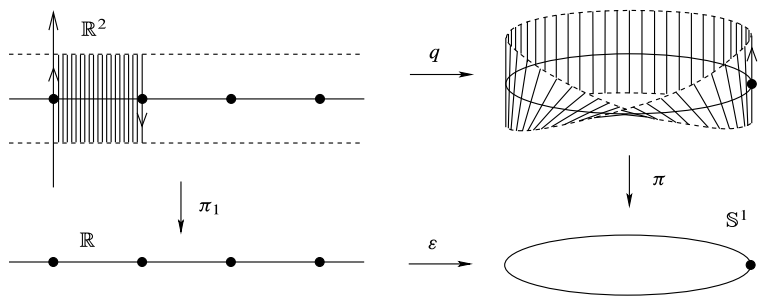
\includegraphics[scale = 0.45]{mobius_bundle.png}}
\end{minipage}
\caption{\scriptsize
\textbf{The M{\"o}bius Bundle. \citep{lee2003introduction} }}
\label{fig: mobius_bundle}
\end{figure}

To visualize $E$, let $S$ denote the strip $[0,1] \times \bR \subset \bR^2$. The restriction of $q$ to $S$ is \emph{surjective} and \emph{closed}, so it is a \emph{quotient map}. The only nontrivial identifications made by $q|_{S}$ are on the \emph{two boundary lines}, so we can think of $E$ as the space obtained from $S$ by giving the right-hand edge a half-twist to turn it upside-down, and then pasting it to the left-hand edge (Fig. \ref{fig: mobius_bundle}). For any $r > 0$, the image under the quotient map $q$ of the rectangle $[0,1] \times [-r,r]$ is \emph{a smooth \textbf{compact manifold} with boundary} called \emph{\textbf{a M\"obius band}}; you can make a paper model of this space by pasting the ends of a strip of paper together with a half-twist.

Consider the following \emph{commutative diagram}:
\[
  \begin{tikzcd}
    \bR^2 \arrow{r}{q} \arrow[swap]{d}{\pi_1} & E \arrow{d}{\pi} \\
    \bR \arrow{r}{\epsilon} & \bS^1,
  \end{tikzcd}
\] where $\pi_1$ is the \emph{\textbf{projection}} onto the \emph{first factor} and $\epsilon: \bR \rightarrow \bS^1$ is the \emph{\textbf{smooth covering map}} $\epsilon(x) = \exp\paren{2\pi\,j x}$. Because $\epsilon \circ \pi_1$ is \emph{\textbf{constant}} on \emph{each equivalence class}, it descends to \emph{\textbf{a continuous map}} $\pi: E \rightarrow \bS^1$.

A straightforward (if tedious) verification shows that $E$ has a \emph{unique smooth manifold structure} such that $q$ is \emph{\textbf{a smooth covering map}} and $\pi: E \rightarrow \bS^1$ is \emph{\textbf{a smooth real line bundle}} over $\bS^1$, called \emph{\textbf{the M{\"o}bius bundle}}. \qed

\end{example}

\item The most important examples of vector bundles are \emph{tangent bundles}.
\begin{proposition} (\textbf{The Tangent Bundle as a Vector Bundle}).\\
 Let $M$ be a smooth $n$-manifold with or without boundary, and let $TM$ be its tangent bundle. With its \textbf{standard projection map}, its \textbf{natural vector space structure} on each \textbf{fiber}, and the \textbf{topology} and \textbf{smooth structure} constructed as in chapter 3, $TM$ is a \textbf{smooth vector bundle} of rank $n$ over $M$.
\end{proposition}
\begin{proof}
Given any smooth chart $(U, \varphi)$ for $M$ with coordinate functions $(x^i)$, define a map $\Phi: \pi^{-1}(U) \rightarrow U \times \bR^n$ by
\begin{align*}
\Phi\paren{v^{i}\partdiff{}{x^{i}}\Bigr|_{p}} &= \paren{p, (v^1, \ldots, v^n)}
\end{align*} This is linear on fibers and satisfies $\pi_1 \circ \Phi = \pi$. The composite map
\begin{align*}
\pi^{-1}(U) \xrightarrow{\Phi} U \times \bR^n \xrightarrow{\varphi \times \text{Id}_{\bR^n}} \varphi(U) \times \bR^{n}
\end{align*} is equal to the coordinate map $\widetilde{\varphi}$ constructed in chapter 3. Since both $\widetilde{\varphi}$ and $\varphi \times \text{Id}_{\bR^n}$ are \emph{diffeomorphisms}, so is $\Phi$. Thus,  $\Phi$ satisfies all the conditions for a smooth local trivialization.  \qed
\end{proof}


\item Another example is \emph{the cotangent bundle} (its fiber is a dual space of tangent space) that will be defined in next chapter.
\begin{proposition} (\textbf{The Cotangent Bundle as a Vector Bundle}).\\
Let $M$ be a smooth $n$-manifold with or without boundary. With its standard projection map and the natural vector space structure on each fiber, the \textbf{cotangent bundle} $T^{*}M$ has a \textbf{unique topology} and \textbf{smooth structure} making it into a \textbf{smooth} \textbf{rank-$n$ vector bundle} over $M$ for which all coordinate covector fields are \textbf{smooth local sections}.
\end{proposition}

\item \begin{example}  (\emph{\textbf{Whitney Sums}}). \\
Given a smooth manifold $M$ and smooth vector bundles $E' \rightarrow M$ and $E'' \rightarrow M$ of ranks $k'$ and $k''$, respectively, we will construct a new vector bundle over $M$ called \emph{\textbf{the Whitney sum}} of $E'$ and $E''$, whose \emph{\textbf{fiber}} at each $p \in M$ is \emph{\textbf{the direct sum}} $E_p' \oplus E_p''$. \emph{The total space} is defined as $E' \oplus E'' = \bigsqcup_{p \in M}E_p' \oplus E_p''$, with the obvious projection $\pi: E' \oplus E'' \rightarrow M$.  For each $p \in M$,  choose a neighborhood $U$ of $p$ small enough that there exist \emph{local trivializations} $(U, \Phi')$ of $E'$ and $(U, \Phi'')$ of $E''$, and define $\Phi: \pi^{-1}(U)  \rightarrow  U \times  \bR^{k' + k''}$ by
\begin{align*}
\Phi(v', v'') &= \paren{\pi'(v'), \paren{\pi_{\bR^{k'}}\circ\Phi'(v'),  \pi_{\bR^{k''}}\circ\Phi''(v'')}}.
\end{align*}

Suppose we are given \emph{another} such pair of \emph{local trivializations} $(\widetilde{U}, \widetilde{\Phi}')$ and $(\widetilde{U}, \widetilde{\Phi}'')$. Let $\tau': (U \cap \widetilde{U}) \rightarrow GL(k', \bR)$ and $\tau'': (U \cap \widetilde{U}'') \rightarrow GL(k'',\bR)$ be the corresponding \emph{transition functions}. Then the \emph{\textbf{transition function}} for $E' \oplus E''$ has the form
\begin{align*}
\widetilde{\Phi} \circ \Phi^{-1}(p, (v', v'')) &= (p, \tau(p)(v', v'')),
\end{align*}
where $\tau(p) = \tau'(p) \oplus \tau''(p) \in GL(k'+ k'', \bR)$ is the \emph{\textbf{block diagonal matrix}}
\begin{align*}
\brac{
\begin{array}{cc}
\tau'(p) & 0 \\
0 & \tau''(p)
\end{array}}.
\end{align*} Because this depends smoothly on $p$, it follows from the chart lemma that $E' \oplus E''$ is a smooth vector bundle over $M$. \qed
\end{example}


\item \begin{example} (\textbf{\emph{Ambient Tangent Bundle}})\\
Suppose $\pi: E \rightarrow M$ is a rank-$k$ vector bundle and $S \subseteq M$ is any subset. We define the \emph{\textbf{restriction of $E$ to $S$}} to be
the set $E|_{S} = \bigcup_{p\in S} E_p$, with the projection $E|_{S} \rightarrow S$ obtained by \textbf{restricting} $\pi$. If $\Phi:  \pi^{-1}(U) \rightarrow U \times \bR^k$ is a \emph{local trivialization} of $E$ over $U \subset M$; it restricts to a \emph{bijective map} $\Phi|_{U}: (\pi|_{S})^{-1}(U \cap S) \rightarrow (U \cap S) \times \bR^k$, and it is easy to check that these form \emph{local trivializations} for a \emph{\textbf{vector bundle structure}} on $E|_{S}$. 
If $E$ is a smooth vector bundle and $S \subseteq M$ is an \emph{immersed} or\emph{ embedded submanifold}, it follows easily from the chart lemma that $E|_{S}$ is a smooth vector bundle. In particular, if $S \subseteq M$ is a \emph{smooth (embedded or immersed) submanifold}, then the \emph{\textbf{restricted bundle}} $TM|_{S}$ is called \emph{the \textbf{ambient tangent bundle} over $M$}. \qed
\end{example}
\end{itemize}
\section{Local and Global Sections of Vector Bundles}
\subsection{Local and Global Sections}
\begin{itemize}

\begin{figure}[htb]
\centering
\begin{minipage}{0.5\linewidth}
 \centerline{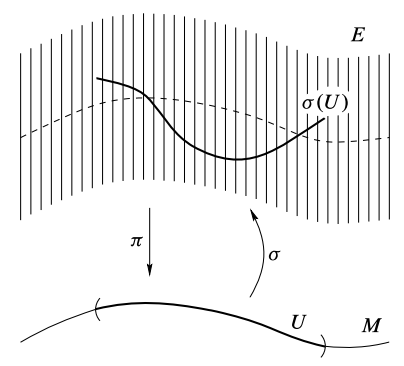
\includegraphics[scale = 0.45]{local_section_vector_bundle.png}}
\end{minipage}
\caption{\scriptsize
\textbf{The local section of vector bundle $E$ over neighborhood $U$. \citep{lee2003introduction} }}
\label{fig: local_section_vector_bundle}
\end{figure}

\item \begin{definition}
Let $\pi: E \rightarrow M$ be a vector bundle. A \underline{\emph{\textbf{section}}} of $E$ (sometimes called \emph{\textbf{a cross section}}) is a \emph{\textbf{section}} of the map $\pi$, that is, a continuous map  $\sigma: M \rightarrow E$ satisfying
\begin{align*}
\pi \circ \sigma =  \text{Id}_M. 
\end{align*} This means that $\sigma(p)$ is an element of the \emph{fiber} $E_p$ for each $p \in M$.
\end{definition}

\item \begin{definition} 
More generally, \emph{\textbf{a \underline{local section} of $E$}} is a \emph{continuous} map $\sigma: U \rightarrow E$ defined on some open subset $U \subseteq M$ and satisfying $\pi \circ \sigma =  \text{Id}_U.$ (See FIg \ref{fig: local_section_vector_bundle}.)

To emphasize the distinction, a section defined on \emph{all of $M$} is sometimes called \emph{\textbf{a global section}}. Note that a \emph{local section} of $E$ over $U \subseteq  M$ is the same as a \emph{global section} of \emph{the \textbf{restricted bundle}} $E|_{U}$.
\end{definition}


\item \begin{definition}
If $M$ is a smooth manifold with or without boundary and $E$ is a \emph{\textbf{smooth vector bundle}}, a \underline{\emph{\textbf{smooth (local or global) section} of $E$}} is one that is a
\emph{smooth map} from its domain to $E$.
\end{definition}

\item \begin{remark}
Just like a \emph{vector bundle} $E$ is a generalization of a \emph{tangent bundle} $TM$, a \emph{\textbf{section}} $\sigma$ \emph{\textbf{of vector bundle}} is a \emph{generalization} of the \emph{\textbf{vector fields}} $X$. $\sigma(p) \in E_p$ is an element of the vector space $E_p$ and $\sigma$ associates  each point in space $M$ with an element of the vector space $E_p$.
\end{remark}

\item \begin{definition}
Define a \emph{\textbf{rough (local or global) section}} of $E$ over a set $U \subseteq M$ to be a map $\sigma: U \rightarrow E$ (\textit{not necessarily continuous}) such that  $\pi \circ \sigma =  \text{Id}_U$. A ``section” without further qualification always means a continuous section.
\end{definition}

\item \begin{definition}
The \emph{\textbf{zero section}} of $E$ is the \textbf{global section} $\xi: M \rightarrow E$ defined by
\begin{align*}
\xi(p) &= 0 \in E_{p}, \quad \forall p \in M.
\end{align*}
\end{definition}

\item \begin{definition}
As in the case of vector fields, the \emph{\textbf{support}} of a section $\sigma$ is the \emph{\textbf{closure} of the set} $\set{p \in M:\;  \sigma(p) \neq 0}$.
\end{definition}

\item \begin{example} (\emph{\textbf{Sections of Vector Bundles}}). \\
Suppose $M$ is a smooth manifold with or without boundary.
\begin{enumerate}
\item Sections of $TM$ are \emph{\textbf{vector fields}} on $M$;
\item Given an \emph{immersed submanifold} $S \subseteq M$ with or without boundary, a section of \emph{\textbf{the ambient tangent bundle}} $TM|_{S} \rightarrow S$ is called \emph{a \textbf{vector field along $S$}}. It is a \emph{continuous} map $X: S \rightarrow TM$ such that $X_p \in T_{p}M$ for each $p \in S$. 

This is different from \emph{a vector field \textbf{on} $S$}, which satisfies $X_p \in T_{p}S$ at each point.
\item If $E = M \times \bR^k$ is a \emph{\textbf{product bundle}}, there is a \textit{natural \textbf{one-to-one correspondence}} between sections of $E$ and continuous functions from $M$ to $\bR^k$: a continuous function $F: M \rightarrow \bR^k$ determines a \emph{\textbf{section}} $\widetilde{F}: M \rightarrow M \times \bR^k$ by $\widetilde{F}(x) = (x, F(x))$, and vice versa. 

If $M$ is a smooth manifold with or without boundary, then the section $\widetilde{F}$ is smooth if and only if $F$ is.
\item  The correspondence in the preceding paragraph yields a natural \textbf{\emph{identification}} between the \emph{space} $\cC^{\infty}(M)$ and \emph{the space of \textbf{smooth sections} of the \textbf{trivial line bundle}} $M \times \bR \rightarrow M$
\end{enumerate}
\end{example}

\item \begin{definition}
If $E \rightarrow M$ is a smooth vector bundle, the set of \emph{\textbf{all smooth global sections of $E$}} is a \emph{\textbf{vector space}} under pointwise addition and scalar multiplication:
\begin{align*}
(c_1 \sigma_1 + c_2 \sigma_2)(p) &= c_1 \sigma_1(p) + c_2 \sigma_2(p)
\end{align*} This vector space is usually \textbf{\emph{denoted by $\Gamma(E)$}}.  Note that for vector fields of tangent bundle $TM$, we use $\mathfrak{X}(M)$
\end{definition}

\item \begin{remark}
Just like smooth vector fields, \emph{smooth sections} of a \emph{smooth bundle} $E \rightarrow M$  can be \emph{multiplied} by \emph{smooth real-valued functions}: if $f \in \cC^{\infty}(M)$ and $\sigma \in \Gamma(E)$, we obtain \emph{a \textbf{new section}} $f\sigma$ defined by
\begin{align*}
(f\sigma)(p) &= f(p)\,\sigma(p).
\end{align*}
\end{remark}

\item \begin{lemma}\label{lem: ext_vector_bundle} (\textbf{Extension Lemma for Vector Bundles}).\\
Let $\pi: E \rightarrow M$ be a smooth vector bundle over a smooth manifold $M$ with or without boundary. Suppose $A$ is a \textbf{closed subset} of $M$, and $\sigma: A \rightarrow E$ is a section of $E|_{A}$ that is \textbf{smooth} in the sense that $\sigma$ \textbf{extends} to a smooth local section of $E$ in a neighborhood of each
point. For each open subset $U \subseteq M$ containing $A$, there exists a \textbf{global smooth section} $\widetilde{\sigma} \in \Gamma(E)$ such that $\widetilde{\sigma}|_{A} = \sigma$ and $\text{supp}(\widetilde{\sigma}) \subseteq U$. 
\end{lemma}
\end{itemize}

\subsection{Local and Global Frames}
\begin{itemize}
\item \begin{definition}
Let $E \rightarrow M$ be a vector bundle. If $U \subseteq M$ is an open subset, a \emph{\textbf{$k$-tuple}} of \emph{\textbf{local sections}} $(\sigma_1,\ldots, \sigma_k)$ of $E$ over $U$ is said to be \emph{\textbf{linearly independent}} if their values $(\sigma_1(p),\ldots, \sigma_k(p))$ form a \emph{linearly independent $k$-tuple in $E_p$} for each $p\in U$. 

Similarly, they are said to \emph{\textbf{span}} $E$ if \emph{their values span $E_p$ for each $p \in U$}.
\end{definition}

\item \begin{definition}
\emph{A \textbf{local frame} for $E$ over $U$} is an ordered $k$-tuple $(\sigma_1,\ldots, \sigma_k)$ of \emph{\textbf{linearly independent} local sections} over U that \emph{\textbf{span}} $E$; thus $(\sigma_1(p),\ldots, \sigma_k(p))$ is a \emph{\textbf{basis}} for the \emph{fiber} $E_p$ for each $p \in U$. 

It is called a \emph{\textbf{global frame}} if $U = M$. 
\end{definition}


\item \begin{definition}
If  $E \rightarrow M$ is a smooth vector bundle, a \emph{local or global frame} is a \emph{\textbf{smooth frame}} if each $\sigma_i$ is a \emph{smooth section}. We often\emph{ denote a frame $(\sigma_1,\ldots, \sigma_k)$ by $(\sigma_i)$}.
\end{definition}


\item \begin{remark}
The \emph{(local or global) frames} for $M$ that we defined in Chapter 8 are, in our new terminology, frames for the tangent bundle. We use both terms interchangeably
depending on context: ``\emph{\textbf{frame for $M$}}" and ``\emph{\textbf{frame for $TM$}}" mean the same thing.
\end{remark}

\item \begin{proposition} (\textbf{Completion of Local Frames for Vector Bundles}). \citep{lee2003introduction} \\
Suppose $\pi: E \rightarrow M$ is a smooth vector bundle of rank $k$.
\begin{enumerate}
\item If $(\sigma_1,\ldots, \sigma_m)$ is a linearly independent $m$-tuple of smooth local sections of $E$ over an open subset $U \subseteq M$, with $1 \le m < k$, then for each $p \in U$ there exist smooth sections $\sigma_{m+1},\ldots, \sigma_{k}$ defined on some neighborhood $V$ of $p$ such that $(\sigma_1,\ldots, \sigma_k)$ is a smooth local frame for $E$ over $U \cap V$.
\item If $(v_1,\ldots,v_m)$ is a linearly independent $m$-tuple of elements of $E_p$ for some $p\in M$, with $1 \le m \le k$, then there exists a smooth local frame $(\sigma_i)$ for $E$ over some neighborhood of $p$ such that $\sigma_i(p) = v_i$ for $i = 1,\ldots,m$.
\item If $A \subseteq M$ is a closed subset and $(\tau_1,\ldots, \tau_k)$ is a linearly independent $k$-tuple of sections of $E|_{A}$ that are smooth in the sense described in Lemma  \ref{lem: ext_vector_bundle}, then there exists a smooth local frame $(\sigma_1,\ldots, \sigma_k)$ for $E$ over some neighborhood of $A$ such that $\sigma_i|_{A} = \tau_i$ for $i = 1,\ldots,k$.
\end{enumerate}
\end{proposition}



\item \begin{remark} (\textbf{\emph{Local Frames Associated with Local Trivializations}}).\\
Suppose $E \rightarrow M$  is a smooth vector bundle. If $\Phi: \pi^{-1}(U) \rightarrow U \times \bR^{k}$ is a smooth local trivialization of $E$, we can construct a local frame for $E$ over $U$.  Define maps $\sigma_1, \ldots, \sigma_k: U \rightarrow E$ by $\sigma_i(p) = \Phi^{-1}(p, e_i) = \Phi^{-1} \circ \widetilde{e}_i(p)$ as below:
\[
  \begin{tikzcd}
    \pi^{-1}(U) \arrow{rr}{\Phi} \arrow{dr}{\pi} &   &U \times \bR^{k} \arrow[swap]{dl}{\pi_1} \\
                                                                            &   U \arrow[ul, bend left, "\sigma_i"]  \arrow[ur, swap, bend right , "\widetilde{e}_i"] &,
  \end{tikzcd}
\]  where $(e_1,\ldots, e_k)$  are the standard basis for $\bR^k$ so that $\widetilde{e}_i$ is the frame such that $\widetilde{e}_i = (p, e_i)$. Then $\sigma_i$ is \textit{smooth} because $\Phi$ is a diffeomorphism, and the fact that $\pi_1 \circ \Phi = \pi$ implies that
\begin{align*}
\pi \circ \sigma_i(p) &=  \pi \circ  \Phi^{-1}(p, e_i) = \pi_1(p, e_i) = p,
\end{align*} so $\sigma_i$ is a \emph{section}. To see that $(\sigma_i(p))$ forms \emph{a basis for $E_p$}, just note that $\Phi$ restricts to an \emph{isomorphism} from $E_p$ to $\set{p} \times \bR^k$, and $\Phi(\sigma_i(p)) = (p, e_i)$, so $\Phi$ takes $\sigma_i(p)$ to the standard basis for $\set{p} \times \bR^k \simeq \bR^{k}$. We say that \emph{\textbf{this local frame $(\sigma_i)$ is associated with $\Phi$}}. \qed
\end{remark}

\item \begin{proposition}
Every \textbf{smooth local frame} for a smooth vector bundle is associated with a \textbf{smooth local trivialization} constructed as above.
\end{proposition}


\item \begin{corollary}
A smooth vector bundle is \textbf{smoothly trivial} if and only if it admits a \textbf{smooth global frame}.
\end{corollary}

\item \begin{corollary} (\textbf{The Coordinate Representation of Vector Bundle})\\
Let  $E \rightarrow M$  be a smooth vector bundle of rank $k$, let $(V, \varphi)$ be a smooth chart on $M$ with coordinate functions $(x^i)$, and suppose there exists a
smooth local frame $(\sigma_i)$ for $E$ over $V$. Define $\widetilde{\varphi}: \pi^{-1}(V) \rightarrow \varphi(V)  \times \bR^k$ by
\begin{align}
\widetilde{\varphi}\paren{v^{i} \sigma_i(p)} &= \paren{x^1(p), \ldots, x^{n}(p), v^1, \ldots, v^{k}}.   \label{eqn: coordinate_representation_vector_bundle_local_frame}
\end{align} Then $(\pi^{-1}(V), \widetilde{\varphi})$ is a \textbf{smooth coordinate chart} for $E$.
\end{corollary}

\item Just as \emph{smoothness} of vector fields can be characterized in terms of their \emph{\textbf{component functions}} in any smooth chart, \emph{smoothness} of sections of vector bundles can be characterized in terms of \emph{\textbf{local frames}}. 

\item \begin{definition} 
Suppose  $(\sigma_i)$ is a smooth local frame for $E$ over some open subset $U \subseteq M$. If $\tau: M \rightarrow E$ is a \emph{rough section}, the value of $\tau$ at
an arbitrary point $p \in U$ can be written $\tau(p) = \tau^{i}(p)\sigma_i(p)$ for some uniquely determined numbers $(\tau^1(p), \ldots, \tau^{k}(p))$. This defines $k$ functions $\tau^i: U \rightarrow \bR$, called \emph{the \textbf{component functions} of $\tau$ with respect to the given local frame}.
\end{definition}

\item \begin{proposition}  (\textbf{Local Frame Criterion for Smoothness}).\\
Let $\pi: E \rightarrow M$ be a smooth vector bundle, and let $\tau: M \rightarrow E$ be a rough section. If  $(\sigma_i)$ is a smooth local frame for $E$ over an open subset $U \subseteq M$, then $\tau$ is smooth on $U$ if and only if its component functions with respect to $(\sigma_i)$ are smooth.
\end{proposition}


\item \begin{proposition} (\textbf{Uniqueness of the Smooth Structure on $TM$})\\
Let $M$ be a smooth n-manifold with or without boundary. The topology and smooth structure on $TM$ constructed in Proposition 3.18 are \textbf{the unique ones} with respect to which $\pi: TM \rightarrow M$ is a \textbf{smooth} vector bundle with the given vector space structure on the fibers, and such that \textbf{all coordinate vector fields are smooth local sections}.
\end{proposition}
\end{itemize}


\section{Bundle Homomorphisms}
\begin{itemize}
\item \begin{definition}
If $\pi: E \rightarrow M$ and $\pi': E' \rightarrow M'$ are vector bundles, a \emph{\textbf{continuous map}} $F: E \rightarrow E'$ is called a \underline{\emph{\textbf{bundle homomorphism}}} if there exists a map $f: M \rightarrow M'$ satisfying $\pi' \circ F = f \circ \pi$,
\[
  \begin{tikzcd}
    E \arrow{r}{F} \arrow{d}{\pi} &  E' \arrow{d}{\pi'} \\
    M                \arrow{r}{f}                                &  M',
  \end{tikzcd}
\] with the property that for each $p \in M$, the \emph{\textbf{restricted map}} $F|_{E_{p}}: E_p \rightarrow E'_{f(p)}$ is \emph{\textbf{linear}}. The \emph{relationship} between $F$ and $f$ is expressed by saying that \underline{\emph{$F$ \textbf{covers} $f$}}.
\end{definition}

\item \begin{remark}
By definition, a bundle \emph{\textbf{homomorphism}} is \emph{not necessary bijective}, unlike the normal \emph{\textbf{homemorphism}} definition.
\end{remark}

\item \begin{proposition}
Suppose $\pi: E \rightarrow M$ and $\pi': E' \rightarrow M'$ are vector bundles and $F: E \rightarrow E'$ is a bundle homomorphism \textbf{covering} $f: M \rightarrow M'$. Then $f$ is \textbf{continuous} and is \textbf{uniquely determined} by $F$. If the bundles and $F$ are all \textbf{smooth}, then $f$ is \textbf{smooth} as well.
\end{proposition}

\item \begin{definition}
A \emph{\textbf{bijective bundle homomorphism}} $F: E \rightarrow E'$ whose \emph{inverse} is also a \emph{bundle homomorphism} is called a \underline{\emph{\textbf{bundle isomorphism}}}; if $F$ is also a \emph{diffeomorphism}, it is called a \underline{\emph{\textbf{smooth bundle isomorphism}}}. If there exists a \emph{(smooth) bundle isomorphism} between $E$ and $E'$, the two bundles are said to be \emph{\textbf{(smoothly) isomorphic}}.
\end{definition}

\item \begin{definition}
\emph{\textbf{A bundle homomorphism over $M$}} is a \emph{bundle homomorphism} covering the
\emph{\textbf{identity map}} of $M$; or in other words, a \emph{continuous} map $F: E \rightarrow E'$ such that
\[
  \begin{tikzcd}
    E \arrow{rr}{F} \arrow[swap]{dr}{\pi} &  & E' \arrow{dl}{\pi'} \\
    & M,              &  
  \end{tikzcd}
\]
and whose \emph{\textbf{restriction to each fiber} is \textbf{linear}}. If there exists a \emph{bundle homomorphism $F: E \rightarrow E'$ over $M$} that is also a \emph{(smooth) bundle isomorphism}, then we say that $E$ and $E'$ are \emph{\textbf{(smoothly) isomorphic over $M$}}. 
\end{definition}

\item The next proposition shows that it is not necessary to check smoothness of the inverse. 
\begin{proposition}
Suppose $E$ and $E'$ are smooth vector bundles over a smooth manifold $M$ with or without boundary, and $F: E \rightarrow E'$ is a \textbf{bijective} \textbf{smooth} \textbf{bundle homomorphism over $M$}. Then $F$ is a smooth bundle \textbf{isomorphism}.
\end{proposition}

\item \begin{example} (\textbf{Bundle Homomorphisms}). \\
\begin{enumerate}
\item If $F: M \rightarrow N$ is a smooth map, \textbf{\emph{the global differential}} $dF: TM \rightarrow TN$ is a \emph{\textbf{smooth bundle homomorphism covering $F$}}.
\item If $E \rightarrow M$ is a smooth vector bundle and $S \subseteq M$ is an \emph{\textbf{immersed submanifold}} with or without boundary, then the \emph{\textbf{inclusion map}} $E|_{S} \xhookrightarrow{} E$ is a \emph{\textbf{smooth bundle homomorphism covering the inclusion of $S$ into $M$}}.
\end{enumerate}
\end{example}

\item \begin{definition}
Suppose $E \rightarrow M$ and $E' \rightarrow M'$ are smooth vector bundles over a smooth manifold $M$ with or without boundary, and let $\Gamma(E)$, $\Gamma(E')$ denote their spaces of smooth global sections. If $F: E \rightarrow E'$ is a \emph{\textbf{smooth bundle homomorphism over $M$}}, then \emph{\textbf{composition with $F$}} \textit{\textbf{induces}} a map $\widetilde{F}: \Gamma(E) \rightarrow \Gamma(E')$ as follows:
\begin{align}
\widetilde{F}(\sigma)(p) &= (F \circ \sigma)(p) = F(\sigma(p)) \label{eqn: bundle_homomorphism_induced_map}
\end{align}
It is easy to check that $\widetilde{F}(\sigma)$ is a \emph{\textbf{section}} of $E'$, and it is \emph{\textbf{smooth}} by composition.
\end{definition}

\item \begin{remark}
Because a \emph{bundle homomorphism} is \emph{\textbf{linear on fibers}}, the resulting map $\widetilde{F}$ on \emph{\textbf{sections}} is \emph{\textbf{linear}} over $\bR$. In fact, it satisfies a stronger linearity property.
\end{remark}

\item \begin{definition}
A map $\cF: \Gamma(E) \rightarrow \Gamma(E')$ is said to be \emph{\textbf{linear over $\cC^{\infty}(M)$}} if for any smooth functions $u_1,u_2 \in \cC^{\infty}(M)$ and smooth sections $\sigma_1, \sigma_2 \in \Gamma(E)$,
\begin{align*}
\cF(u_1\sigma_1 + u_2\sigma_2) &= u_1 \cF(\sigma_1) + u_2\cF(\sigma_2).
\end{align*}
\end{definition}


\item It follows easily from the definition \eqref{eqn: bundle_homomorphism_induced_map} that the map on sections induced by a \emph{smooth bundle homomorphism} is \emph{\textbf{linear} over $\cC^{\infty}(M)$}. The next lemma shows that the converse is true as well.
\begin{lemma} (\textbf{Bundle Homomorphism Characterization Lemma}). \citep{lee2003introduction}\\
Let $\pi: E \rightarrow M$ and $\pi': E' \rightarrow M'$ be smooth vector bundles over a smooth manifold $M$ with or without boundary, and let $\Gamma(E)$, $\Gamma(E')$ denote their spaces of smooth sections. A map $\cF: \Gamma(E) \rightarrow \Gamma(E')$ is \textbf{linear over $\cC^{\infty}(M)$} \textbf{if and only if} there is a \textbf{smooth bundle homomorphism} $F: E \rightarrow E'$ over $M$ such that $\cF(\sigma) = F\circ \sigma$ for all $\sigma \in \Gamma(E)$.
\end{lemma}

\item \begin{example} (\emph{\textbf{Bundle Homomorphisms Over Manifolds}}). \\
\begin{enumerate}
\item If $M$ is a smooth manifold and $f \in \cC^{\infty}(M)$, the map from $\frX(M)$ to itself defined by $X \mapsto fX$ is linear over  $\cC^{\infty}(M)$ because $f (u_1\,X_1 + u_2\,X_2) =  u_1\,f(X_1) + u_2\,f(X_2)$, and thus defines \emph{\textbf{a smooth bundle homomorphism}} over $M$ from $TM$ to itself.
\item If $Z$ is a smooth vector field on $\bR^3$, the \emph{\textbf{cross product}} with $Z$ defines a map from $\frX(\bR^3)$ to itself: $X \mapsto X \times Z$. Since it is linear over $\cC^{\infty}(\bR^3)$ in $X$, it determines \emph{a \textbf{smooth bundle homomorphism} over $\bR^3$} from $T\bR^3$ to $T\bR^3$.
\item Given $Z \in \frX(\bR^n)$, the \emph{\textbf{Euclidean dot product}} defines a map $X \mapsto X \cdot Z$ from $\frX(\bR^n)$ to $\cC^{\infty}(\bR^n)$, which is linear over $\cC^{\infty}(\bR^n)$ and thus determines \emph{a \textbf{smooth bundle homomorphism} over $\bR^n$} from $T\bR^n$ to the \emph{trivial line bundle} $\bR^n \times \bR$.
\end{enumerate}
\end{example}

\item \begin{remark}
Because of \emph{Bundle Homomorphism Characterization Lemma}, we usually dispense with the notation $\widetilde{F}$ and use \emph{\textbf{the same symbol}} for both \emph{\textbf{a bundle homomorphism}} $F: E \rightarrow E'$ over $M$ and \emph{\textbf{the linear map}} $F: \Gamma(E) \rightarrow \Gamma(E')$ that it induces on \emph{\textbf{sections}}, and we refer to a map of \emph{\textbf{either} of these types} as \emph{\textbf{a bundle homomorphism}}.
\end{remark}
\end{itemize}

\section{Subbundles}

%\section{Fiber Bundles}

\newpage
\section{Comparison of concepts}
\begin{itemize}
\item By far, we have introduced a lot of abstract concepts that are generalization of our known concepts. Let us compare them in the following Table \ref{tab: concepts}.

\begin{table}[h!]
\centering
\caption{Comparison between concepts}
\label{tab: concepts}
%\setlength{\extrarowheight}{1pt}
\renewcommand\tabularxcolumn[1]{m{#1}}
\footnotesize
\begin{tabularx}{1\textwidth} { 
  | >{\raggedright\arraybackslash} m{2cm}
  | >{\centering\arraybackslash}X
  | >{\centering\arraybackslash}X
  | >{\centering\arraybackslash}X  | }
 \hline
 base & \emph{\textbf{Euclidean space}} $\bR^{n}$ & \emph{\textbf{smooth manifold}} $M$ & \emph{\textbf{topological space}} $M$  \\
 \hline
 element  & $p$, \textbf{global coordinate} $\mb{x} = (x^1, \ldots, x^{n})$  & $p$, \textbf{local coordinate} $\varphi(p) = (x^1, \ldots, x^{n})$ & $p$\\
\hline
 basis of base & coordinate vectors
$\mb{e}_1, \ldots, \mb{e}_{n}$  & the \emph{local frame} for $M$ & the \emph{local frame} for $M$ \\
\hline
vector space (fiber) at $p$ & tangent space $T_{\mb{x}}\bR^{n}  \simeq \set{\mb{x}} \times \bR^{n} \simeq \bR^{n}$ &  \textbf{tangent space}  $T_{p}M \simeq \set{p} \times \bR^{n}$ & \textbf{fiber} $E_{p} = \pi^{-1}(p)$; $E_{p}  \simeq \set{p} \times \bR^{k} \simeq \bR^{k}$ \\
\hline
dimension of vector space & $n$ & $n$ & $k$ \\
\hline
basis of vector space &

\begin{center}
 \begin{align*}
 \paren{\dfrac{\partial}{\partial x^{1}}\Bigr|_{p}, \ldots, \dfrac{\partial}{\partial x^{n}}\Bigr|_{p}}  \equiv  \\
(\mb{e}_1, \ldots, \mb{e}_{n})
\end{align*} 
 \end{center} &  \begin{align*}
 \paren{\dfrac{\partial}{\partial x^{1}}\Bigr|_{p}, \ldots, \dfrac{\partial}{\partial x^{n}}\Bigr|_{p}}
\end{align*} &   \begin{align*}
 (\sigma_1(p), \ldots, \sigma_{k}(p))
\end{align*} \\
\hline
element in vector space &  \begin{align*}
\text{tangent vector }\\
 \mb{v} = v^{i}\mb{e}_{i}
 \end{align*}  & \begin{align*} 
\text{\textbf{tangent vector} }\\
  v = v^{i}\dfrac{\partial}{\partial x^{i}}\Bigr|_{p}
 \end{align*}  & \begin{align*} 
 v = v^{i}\sigma_{i}(p)
 \end{align*}\\
\hline
total space of bundle & \begin{align*}
\text{tangent bundle }\\
 T\bR^{n} \simeq  \bR^{n} \times \bR^{n}
 \end{align*}  & \begin{align*}
 \text{\textbf{tangent bundle} }\\
TM =  \bigsqcup_{p\in M}T_{p}M
 \end{align*} 
 & 
\begin{align*}
 \text{\textbf{vector bundle} }\\
E =  \bigsqcup_{p\in M}E_{p}, 
 \end{align*}\\
\hline
element in bundle & $(x^1,\ldots, x^{n}, v^1, \ldots, v^{n})$ &
$(x^1(p), \ldots, x^{n}(p),  v^1, \ldots, v^{n})$
& 
$(x^1(p), \ldots, x^{n}(p),  v^1, \ldots, v^{k})$ \\
\hline
section & 
\begin{align*}
\text{\textbf{global vector field} }\\
X = X^{i}\mb{e}_{i} \equiv X^{i}\partdiff{}{x^{i}}
\end{align*} &  
\begin{align*}
\text{\textbf{local vector field} }\\
X = X^{i}\partdiff{}{x^{i}}\\
X_{p} \in T_{p}M
\end{align*}
& \begin{align*}
\text{\textbf{local section} }\\
\tau = \tau^{i}\sigma_{i}\\
\tau(p) \in E_{p}
\end{align*} \\
\hline
vector space of sections & $\mathfrak{X}(\bR^{n}) \simeq \bR^{n}$ & $\mathfrak{X}(M) \equiv \Gamma(TM)$ & $\Gamma(E)$ \\
\hline
frame &
\begin{align*}
\text{\textbf{global frame}}\\
\paren{\mb{e}_1, \ldots, \mb{e}_{n}}
\end{align*} 
&
\begin{align*}
\text{\textbf{basis vector fields}}\\
\paren{\partdiff{}{x^{1}}, \ldots, \partdiff{}{x^{n}}}
\end{align*} &
\begin{align*}
\text{\textbf{local frame}}\\
\paren{\sigma_1, \ldots, \sigma_{k}}
\end{align*} \\
\hline
\end{tabularx}
\end{table}
\end{itemize}



\newpage
\bibliographystyle{plainnat}
\bibliography{book_reference.bib}
\end{document}